\section{Camera Geometry}
We have already seen that the camera is a projection device. The location of the pixel in the image plane has a direct relationship
with the location of the point in the 3D world. When we approximate the camera with a pinhole model, we might lose some information about the scene,
such as the depth of the objects.

The position of the acquisition device plays a crucial role in the way we perceive the world. In this section we will try to give some
explanation of these phenomena and try to give an explanation of how the camera geometry works.

\subsection{2D Case}
Typically, a pixel is represented as a 2D point in the image plane using its coordinates.
\[ p = \begin{bmatrix} x, y \end{bmatrix}^T  = \begin{bmatrix} x \\ y \end{bmatrix} \]

Often, we use homogeneous coordinates to represent points in the image plane. This allows us to represent points at infinity and perform projective transformations more easily. In homogeneous coordinates, a point is represented as a three-dimensional vector:
\[ p = \begin{bmatrix} sx, sy, s \end{bmatrix}^T \]
where \( s \) is a scaling factor, commonly set to 1.

\subsubsection{Affine Transformation}
An affine transformation is a spatial transformation, represented as a multiplication of the \textbf{homogeneous point} with some predefined matrix.
We can define different types of transformations, such as \textbf{scaling}, \textbf{rotation}, \textbf{translation} and a \textbf{composition} of them.

\paragraph{Scaling}
Scaling is a transformation that changes the size of an object, by multiplying the coordinates of each point by a scaling factor $c$. It is applied to all points in the image either uniformly or non-uniformly.
The scaling transformation matrix $S_{c_x, c_y}$ is defined as:
\[ S_{c_x, c_y} = \begin{bmatrix} c_x & 0 \\ 0 & c_y \end{bmatrix} \]

where \( c_x \) and \( c_y \) are the scaling factors for the x and y directions, respectively. 
If the scaling factors are the same, the transformation is uniform.

The new coordinates \( (x', y') \) of the point after scaling can be calculated as:
\[\begin{bmatrix} x' \\ y' \end{bmatrix} = \begin{bmatrix} c_x & 0 \\ 0 & c_y \end{bmatrix} \begin{bmatrix} x \\ y \end{bmatrix} \]

We can express the new coordinates \( (x', y') \) of the point after scaling as:
\[ x' = c_x \cdot x \]
\[ y' = c_y \cdot y \]

\paragraph{Rotation}
Rotation is a transformation that changes the orientation of an object by rotating it around a specific point, usually the origin.

The rotation transformation matrix $R_{\theta}$ for a rotation by an angle \( \theta \) is defined as:
\[ R_{\theta} = \begin{bmatrix} \cos \theta & -\sin \theta \\ \sin \theta & \cos \theta \end{bmatrix} \]
where \( \theta \) is the angle of rotation in radians.

The rotation transformation can be applied to a point \( (x, y) \) in the image plane to obtain the new coordinates \( (x', y') \) after rotation:
\[\begin{bmatrix} x' \\ y' \end{bmatrix} = \begin{bmatrix} \cos \theta & -\sin \theta \\ \sin \theta & \cos \theta \end{bmatrix} \begin{bmatrix} x \\ y \end{bmatrix} \]
The new coordinates \( (x', y') \) of the point after rotation can be calculated as:
\[ x' = x \cdot \cos \theta - y \cdot \sin \theta \]
\[ y' = x \cdot \sin \theta + y \cdot \cos \theta \]

\paragraph{Translation}
Translation is a transformation that moves an object from one location to another without changing its shape or orientation, 
It is represented as a \textbf{shift} in the coordinates of the points in the image, equivalent to changing the origin of the coordinate system.

We basically want to move the point \( (x, y) \) to a new location \( (x', y') \) by adding a translation vector \( (x_0, y_0) \):
\[ x' = x + x_0 \]
\[ y' = y + y_0 \]
To do this, we can represent the translation transformation using homogeneous coordinates, which allows us to express it as a matrix multiplication.
The translation transformation matrix $D_{x_0, y_0}$ can be represented as:
\[ D_{x_0, y_0} = \begin{bmatrix} 1 & 0 & x_0 \\ 0 & 1 & y_0 \\ 0 & 0 & 1 \end{bmatrix} \]

The new coordinates \( (x', y') \) of the point after translation can be calculated as:
\[\begin{bmatrix} x' \\ y' \\ 1 \end{bmatrix} = \begin{bmatrix} 1 & 0 & x_0 \\ 0 & 1 & y_0 \\ 0 & 0 & 1 \end{bmatrix} \begin{bmatrix} x \\ y \\ 1 \end{bmatrix} \]
where \( x_0 \) and \( y_0 \) are the translation distances in the x and y directions, respectively.

\subsubsection{Camera Matrix}
All the transformations we have seen so far can be combined into a single transformation matrix, called the \textbf{camera matrix}. 
This allows us to represent the relationship between the 3D world and the 2D image plane in a compact form, allowing 
to correctly map points from the 3D world to the 2D image plane.

The camera matrix is typically a combination of 4 parameters: rotation angle, translation vector, and the scaling factor. 
\begin{figure}[H]
    \centering
    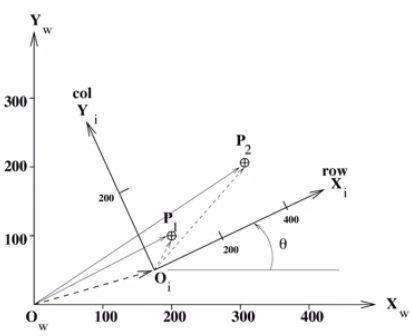
\includegraphics[width=0.5\textwidth]{../media/geometry/2D-camera_matrix.png}
    \caption{Camera matrix in the 2D case.}
\end{figure}
From the example, we can see how the point $P_1$, from the real world, is projected onto the image plane $X_i, Y_i$ as the point $P_2$.
This is done by applying a translation from the real world coordinates to the camera coordinates, 
then applying a rotation of angle $\theta$ and finally applying a scaling factor $s$ to get the final coordinates of the point in the image plane. 

Given a point \( P_j \) in the real world, we can express the transformation to the image plane as follows:
\[ P_j = D_{x_0, y_0} R_{\theta} S_{s_x, s_y} P_i \]
where \( P_i \) is the point in the image plane, \( D_{x_0, y_0} \) is the translation matrix, \( R_{\theta} \) is the rotation matrix, and \( S_{s_x, s_y} \) is the scaling matrix.

\paragraph{Compute the Camera Matrix}
We can compute the parameters of the camera matrix by using a set of known points, called \textbf{control points} in the real world and their 
corresponding points in the image plane.

Since we have 4 parameters to estimate, we need at least 4 equations to solve for these parameters. Each control point
provides us with 2 equations (one for the x-coordinate and one for the y-coordinate), so we need at least 2 control points.

For each control point, we can write the following equations:
\[ \begin{bmatrix}
    x_w \\ y_w \\
\end{bmatrix}
=\begin{bmatrix}
    1 & 0 & x_0 \\
    0 & 1 & y_0 \\
    0 & 0 & 1
\end{bmatrix}
\begin{bmatrix}
    c_x & 0 & 0 \\
    0 & c_y & 0 \\
    0 & 0 & 1
\end{bmatrix}
\begin{bmatrix}
    \cos \theta & -\sin \theta & 0 \\
    \sin \theta & \cos \theta & 0 \\
    0 & 0 & 1
\end{bmatrix}
\begin{bmatrix}
    x_i \\ y_i \\ 1
\end{bmatrix} \]
where \( (x_w, y_w) \) are the coordinates of the point in the real world, 
\( (x_i, y_i) \) are the coordinates of the point in the image plane, 
\( (x_0, y_0) \) are the translation parameters, 
\( (c_x, c_y) \) are the scaling parameters, 
and \( \theta \) is the rotation angle.

\subsubsection{General Camera Matrix}
Given that the three matrices that we are multiplying ($R_{\theta}, S_{s_x, s_y}, D_{x_0, y_0}$) are all of the same size,
we can combine them into a \textbf{single camera matrix} \( C \):
\[ C = \begin{bmatrix}
    a_{11} & a_{12} & a_{13} \\
    a_{21} & a_{22} & a_{23} \\
    0 & 0 & 1
\end{bmatrix} \]

Given the camera matrix \( C \), we can compute the transformation from the real world to the image plane and vice versa.
For example, given a point \( P_j = \begin{bmatrix} x_j \\ y_j \\ 1 \end{bmatrix} \) in the real world, we can compute its projection on the image plane as follows:
\[ P_i = C P_j \]

\paragraph{Least Square Approach}
To obtain the 6 parameters of the camera matrix \( C \), we need at least 3 control points. 
A good rule of thumb is to select them in a way that they are not collinear or too close to each other, to avoid numerical instability in the estimation of the parameters.
But, a more effective way to reduce the error in the estimation of the camera matrix is to use more than 3 control points and solve for the parameters using a least squares approach.

Our goal is to find the set of parameters that minimizes the \textbf{error} between the projected points and the actual points in the image plane.
The error can be defined as the sum of the squared distances between the projected points and the actual points in the image plane:
\[ E = \sum_{j=1}^{N} (a_{11} x_j + a_{12} y_j + a_{13} - u_j)^2 + (a_{21} x_j + a_{22} y_j + a_{23} - v_j)^2 \]
where \( (u_j, v_j) \) are the coordinates of the point in the image plane corresponding to the control point \( P_j = \begin{bmatrix} x_j & y_j & 1 \end{bmatrix} \) in the real world.

The solution to this optimization problem can be found by computing the partial derivatives of the error function with respect to the parameters of the camera matrix,
setting them to zero, and solving the resulting system of equations.

The resulting equation system is:
\[ \begin{bmatrix}
    \sum x_j^2 & \sum x_j y_j & \sum x_j & 0 & 0 & 0 \\
    \sum x_j y_j & \sum y_j^2 & \sum y_j & 0 & 0 & 0 \\
    \sum x_j & \sum y_j & N & 0 & 0 & 0 \\
    0 & 0 & 0 & \sum x_j^2 & \sum x_j y_j & \sum x_j \\
    0 & 0 & 0 & \sum x_j y_j & \sum y_j^2 & \sum y_j \\
    0 & 0 & 0 & \sum x_j & \sum y_j & N
\end{bmatrix}
\begin{bmatrix}
    a_{11} \\ a_{12} \\ a_{13} \\ a_{21} \\ a_{22} \\ a_{23}
\end{bmatrix} =
\begin{bmatrix}
    \sum x_j u_j \\ \sum y_j u_j \\ \sum u_j \\ \sum x_j v_j \\ \sum y_j v_j \\ \sum v_j
\end{bmatrix} \]
This system of equations can be solved using standard linear algebra techniques, such as Gaussian elimination or singular value decomposition, to find the parameters of the camera matrix \( C \).

\subsection{3D Case}
What we have seen so far is a simplified version of the camera geometry, where we have only considered the 2D case.
This was only applicable to the case where the camera is looking at a flat surface, which is perfectly parallel to the image plane. 

In the real world, we usually have a 3D scene and the camera is looking at it from a certain point of view. In this case, we also need to consider
the \textbf{calibration} of the camera, which is the process of estimating the \textbf{intrinsic} parameters of the camera, and the \textbf{extrinsic} parameters.

\subsubsection{Calibration}
As we just said, we need to consider both intrinsic and extrinsic parameters of the camera to correctly model the camera geometry in the 3D case.

\paragraph{Intrinsic} set of parameters that describe the internal characteristics of the camera, and are specific to the sensor itself.
They include parameters such as the focal length, image distortion, and the size of the pixels.

These parameters are crucial for accurately modeling the 3D geometry of the scene. In fact, since each camera has its own intrinsic parameters,
they will affect the outcome of the projection of the 3D points onto the image plane.

\paragraph{Extrinsic} set of parameters that describe the position and orientation of the camera in the 3D world. 
They include parameters such as the rotation and translation of the camera with respect to a reference coordinate system.

Calibration is the process of estimating both intrinsic and extrinsic parameters of the camera, that allow us to correctly
map the 3D points in the world to the 2D points in the image plane.

\subsubsection{3D representation}
In the 3D case, we can represent a point in the world as a 3D vector:
\[ P = \begin{bmatrix} X, Y, Z \end{bmatrix}^T \]
where \( X, Y, Z \) are the coordinates of the point in the 3D space.

We can also represent the point in homogeneous coordinates as:
\[ P = \begin{bmatrix} sX, sY, sZ, s \end{bmatrix}^T \]
where \( s \) is a scaling factor, commonly set to 1.

In general, each point has 4 coordinates systems:
\begin{itemize}
    \item \textbf{Model coordinate system}: the coordinate system defined by the 3D model of the scene, with the origin at a specific point in the scene and the axes aligned with the model;
    \item \textbf{World coordinate system}: the real-world coordinate system;
    \item \textbf{Camera 1 coordinate system}: the coordinate system defined by one camera;
    \item \textbf{Camera 2 coordinate system}: the coordinate system defined by another camera;
\end{itemize}
Since the two cameras can have opposite views of the scene, there is no guarantee that there exists 
a one-to-one mapping for all the points in the scene. 
In fact, some points might be visible in one camera and not in the other, due to occlusions or the limited field of view of the cameras.
For this kind of points, we cannot find their corresponding points in the 3D space.

\subsubsection{3D affine transformation}
Similar to the 2D case, we can also define affine transformations in the 3D case.
The main difference is that we need to consider the z-coordinate of the points in the 3D space, 
and the transformation matrices will be of size 4x4 instead of 3x3.

\note{In the following section we will use a slightly different notation from the previous one.
In particular, we represent as:
\[^kP_i\]
the pixel \( P_i \) in the coordinate system of the camera \( k \).}
\paragraph{Translation}
The translation transformation, mapping a point \( ^1P_i \) in the coordinate system of camera 1 to a point \( ^2P_i \) in the coordinate system of camera 2, can be represented as:

\[ ^2P_i = T(t_x, t_y, t_z) ^1P_i \]
where \( T(t_x, t_y, t_z) \) is the translation matrix defined as:
\[ T(t_x, t_y, t_z) = \begin{bmatrix}
    1 & 0 & 0 & t_x \\
    0 & 1 & 0 & t_y \\
    0 & 0 & 1 & t_z \\
    0 & 0 & 0 & 1
\end{bmatrix} \]
where \( (t_x, t_y, t_z) \) are the translation distances in the x, y, and z directions, respectively.

\paragraph{Scaling}
The scaling transformation, mapping a point \( ^1P_i \) in the coordinate system of camera 1 to a point \( ^2P_i \) in the coordinate system of camera 2, can be represented as:
\[ ^2P_i = S(s_x, s_y, s_z) ^1P_i \]
where \( S(s_x, s_y, s_z) \) is the scaling matrix defined as:
\[ S(s_x, s_y, s_z) = \begin{bmatrix}
    s_x & 0 & 0 & 0 \\
    0 & s_y & 0 & 0 \\
    0 & 0 & s_z & 0 \\
    0 & 0 & 0 & 1
\end{bmatrix} \]
where \( (s_x, s_y, s_z) \) are the scaling factors in the x, y, and z directions, respectively.

\paragraph{Rotation}
The rotation transformation needs to consider the three angles of rotation around the x, y, and z axes.

The rotation transformation, mapping a point \( ^1P_i \) in the coordinate system of camera 1 to a point \( ^2P_i \) in the coordinate system of camera 2, can be represented as:
\begin{itemize}
    \item Rotation around the x-axis:
    \[ ^2P_i = R(X, \theta_x) ^1P_i \]
    where \( R(X, \theta_x) \) is the rotation matrix defined as:
    \[ R(X, \theta_x) = \begin{bmatrix}
        1 & 0 & 0 & 0 \\
        0 & \cos \theta_x & -\sin \theta_x & 0 \\
        0 & \sin \theta_x & \cos \theta_x & 0 \\
        0 & 0 & 0 & 1
    \end{bmatrix} \]
    where \( \theta_x \) is the angle of rotation around the x-axis in radians.
    \item Rotation around the y-axis:
    \[ ^2P_i = R(Y, \theta_y) ^1P_i \]
    where \( R(Y, \theta_y) \) is the rotation matrix defined as:
    \[ R(Y, \theta_y) = \begin{bmatrix}
        \cos \theta_y & 0 & \sin \theta_y & 0 \\
        0 & 1 & 0 & 0 \\
        -\sin \theta_y & 0 & \cos \theta_y & 0 \\
        0 & 0 & 0 & 1
    \end{bmatrix} \]
    where \( \theta_y \) is the angle of rotation around the y-axis in radians.
    \item Rotation around the z-axis:
    \[ ^2P_i = R(Z, \theta_z) ^1P_i \]
    where \( R(Z, \theta_z) \) is the rotation matrix defined as:
    \[ R(Z, \theta_z) = \begin{bmatrix}
        \cos \theta_z & -\sin \theta_z & 0 & 0 \\
        \sin \theta_z & \cos \theta_z & 0 & 0 \\
        0 & 0 & 1 & 0 \\
        0 & 0 & 0 & 1
    \end{bmatrix} \]
    where \( \theta_z \) is the angle of rotation around the z-axis in radians.
\end{itemize}

\subsubsection{General Transformation Matrix}
Similar to the 2D case, we can also define a general camera matrix in the 3D case, which combines all the transformations we have seen so far into a single matrix.
The general camera matrix \( C \) can be represented as:
\[ C = \begin{bmatrix}
    r_{11} & r_{12} & r_{13} & t_x \\
    r_{21} & r_{22} & r_{23} & t_y \\
    r_{31} & r_{32} & r_{33} & t_z \\
    0 & 0 & 0 & 1
\end{bmatrix} \]
This matrix allows us to represent the transformation from real from camera 1 points  \( ^1P_i \) to camera 2 points  \( ^2P_i \)  as follows:
\[ ^2P_i = C ^1P_i \]

\subsubsection{Camera Model}
The General Transformation Matrix \( C \) is a powerful tool to represent the transformation between different camer coordinate systems, 
but it doesn't allow to map points from the 3D world to the 2D image plane, since it doesn't consider the intrinsic parameters of the camera.

To do this, we need to define a camera model that combines both the intrinsic and extrinsic parameters of the camera.
Given the matrix $^I_WC$, we can map points from the world coordinate system $^WP$ to the image plane $^IP$ as follows:
\[ ^IP = ^I_WC ^WP \]
where \( ^I_WC \) is the camera matrix that combines both intrinsic and extrinsic parameters of the camera, and \( ^WP \) is the point in the world coordinate system.

Formally, this transformation can be represented as:
\[ \begin{bmatrix}
    s' P_x \\ s' P_y \\ s'
\end{bmatrix} =
^I_WC \begin{bmatrix}
    ^WP_x \\ ^WP_y \\ ^WP_z \\ 1
\end{bmatrix} \]

\subsubsection{}
The previously defined camera model is a simplified version of the real camera model, which is based on the pinhole camera model.
In fact, the points in the real world are considered as continuous, while the points in the image plane are discrete, since they are represented as pixels.

